\documentclass[UTF8]{ctexart}

\usepackage{mathtools,mathabx,bm,lmodern}
\usepackage{booktabs,siunitx,xltxtra}
\usepackage{datetime}
\usepackage[a4paper,hmargin=1.2in,vmargin=1in]{geometry}
\usepackage{graphicx,tikz,wrapfig}
\usepackage{fancyhdr}
\usepackage{subfigure}
\usepackage{float}
\usepackage{footnote}
\usepackage{listings}
\usepackage{array,tabularx}
\usepackage{verbatim}%多行注释
\usepackage{ragged2e} 
\usepackage{booktabs,makecell, multirow, tabularx}
\usepackage{caption}
\usepackage{multicol}
%\usepackage{bibtex}
\usepackage[utf8]{inputenc}

\usepackage{tikz,mathpazo,xcolor}
\usetikzlibrary{arrows.meta}%箭头
\usepackage{mhchem,chemfig,extarrows}  %化学式
\usepackage{geometry}
\geometry{a4paper,centering,scale=0.9}

\title{原子力显微镜实验报告}
\author{PB22020469 文义钧}

\begin{document}
\maketitle

\section{摘要} 
本实验利用原子力显微镜(AFM)对样品的表面进行微观结构的表征和分析。通过探针与样品表面之间的相互作用,AFM 能够以高分辨率成像并定量测量表面粗糙度、形貌以及局部力学特性。本实验的主要目标是使用轻敲模式对不同材料样品进行表面形貌的测量,并评估其纳米尺度下的特性。实验结果表明,AFM 能够有效表征样品的微观结构,并揭示出其表面细节,如纳米尺度的颗粒、台阶及缺陷。这些结果为进一步的材料性能分析提供了重要的依据。
\section{引言}
原子力显微镜(Atomic Force Microscope, AFM)是一种以物理学原理为基础,通过扫描探针与样品表面原子的相互作用而成像的新型表面分析仪器. 与常规显微镜比较,原子力显微镜的优点是在大气条件下,以高倍率观察样品表面,可用于几乎所有样品(对表面光洁度有一定要求),而不需要进行其他制样处理,就可以得到样品表面的三维形貌图象。并可对扫描所得的三维形貌图象进行粗糙度计算、厚度、步宽、方框图或颗粒度分析。\par

AFM 的工作原理是通过细微的探针扫描样品表面,并利用探针与样品之间的作用力来获得表面形貌信息。探针尖端在小的轫性的悬臂上,当探针接触到样品表面时,产生的相互作用,以悬臂偏转形式检测。样品表面与探针之间的距离小于$3\sim4 \rm nm$,以及在它们之间检测到的作用力,小于 $10^{-8} \rm N$。激光二极管的光线聚焦在悬臂的背面上。当悬臂在力的作用下弯曲时,反射光产生偏转,使用位敏光电检测器检测偏转角。然后通过计算机对采集到的数据进行处理,从而得到样品表面的三维图象。\par

AFM 具有多种工作模式,如接触模式、非接触模式及轻敲模式. 下图显示了AFM各种扫描模式与对应的范德华力的关系和各种工作模式的示意.\\
\begin{minipage}[!ht]{1\linewidth}
    \centering
    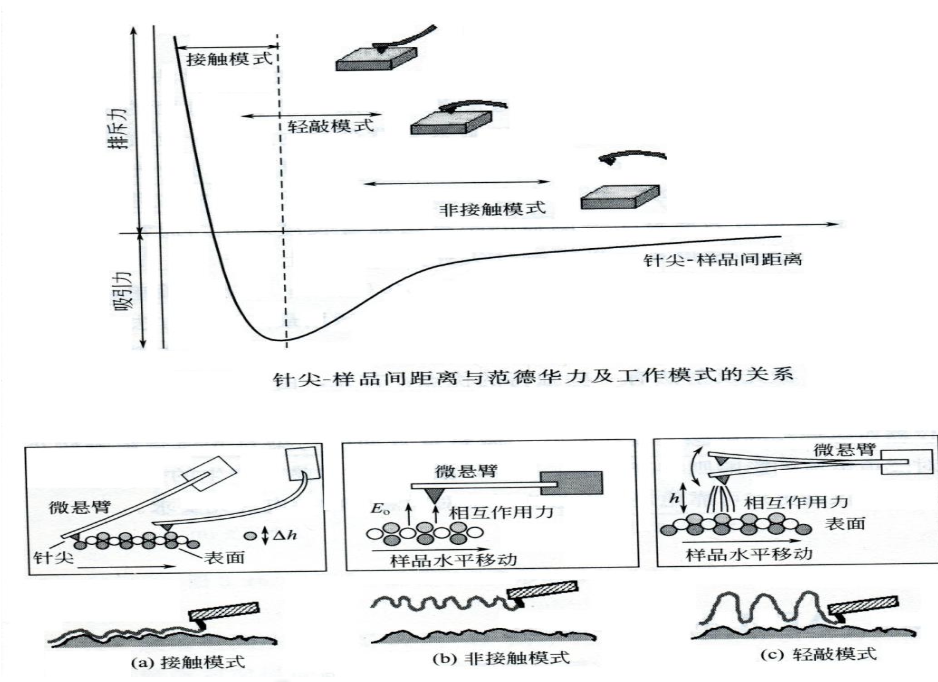
\includegraphics[width=0.7\textwidth]{1.png}\\
    {\small{
        图1. AFM三种工作模式
    }}
    \vspace{10pt}
\end{minipage}\par
近年来原子力显微镜也取得不少突破, 例如筑波大学开发了一种时间分辨的原子力显微镜, 可以捕捉纳米级的超快光诱导现象. 这一技术使可以通过AFM研究极短时间尺度的高精度动态现象.$\rm ^{[2]}$ University of Illinois利用深度学习的AI技术, 大幅提升了显微镜图像的解码能力, 可以自动识别解读显微图像的结构.$\rm ^{[3]}$
\section{实验仪器}
CSPM5500 型扫描探针显微镜,Pt-Ir 合金丝、0.250 μm 的钨丝, 金薄膜(团簇)样品.
\section{实验过程}
\begin{enumerate}
    \item 打开电脑电源、控制箱电源;
    \item 检查光斑状态, 调节螺杆使激光光斑落在光斑位置探测器的小圆圈中央;
    \item 调节扫描参数. 设定共振曲线, 先选择全范围再逐渐缩小区间寻找共振频率;
    \item 确定探针振动频率(斜率最大且最接近共振峰, 振幅约为共振峰的$75\%\sim 95\%$),和参考点(共振曲线斜率最大值处, 振幅约为$50\%\sim70\%$), 并调节红色游标至探针振动频率范围, 输入参考点;
    \item 先自动进针, 逼近样品后选择单步前进/单步后退使得电压读数在$0\rm V$左右;
    \item 确定灵敏度; 调节扫描参数, 调节信号放大和伸缩范围等参数, 使示波器的扫描信号线比较重合且噪音较低;
    \item 扫描并保存扫描结果;
    \item 退针并关闭各个电源.
\end{enumerate}
\section{实验结果}
测量样品表面的原子力显微2D灰度图像如图2所示, 3D形态图如图3所示, 振幅和相移图像如图4,图5所示.\\
\begin{minipage}[!ht]{0.5\linewidth}
    \centering
    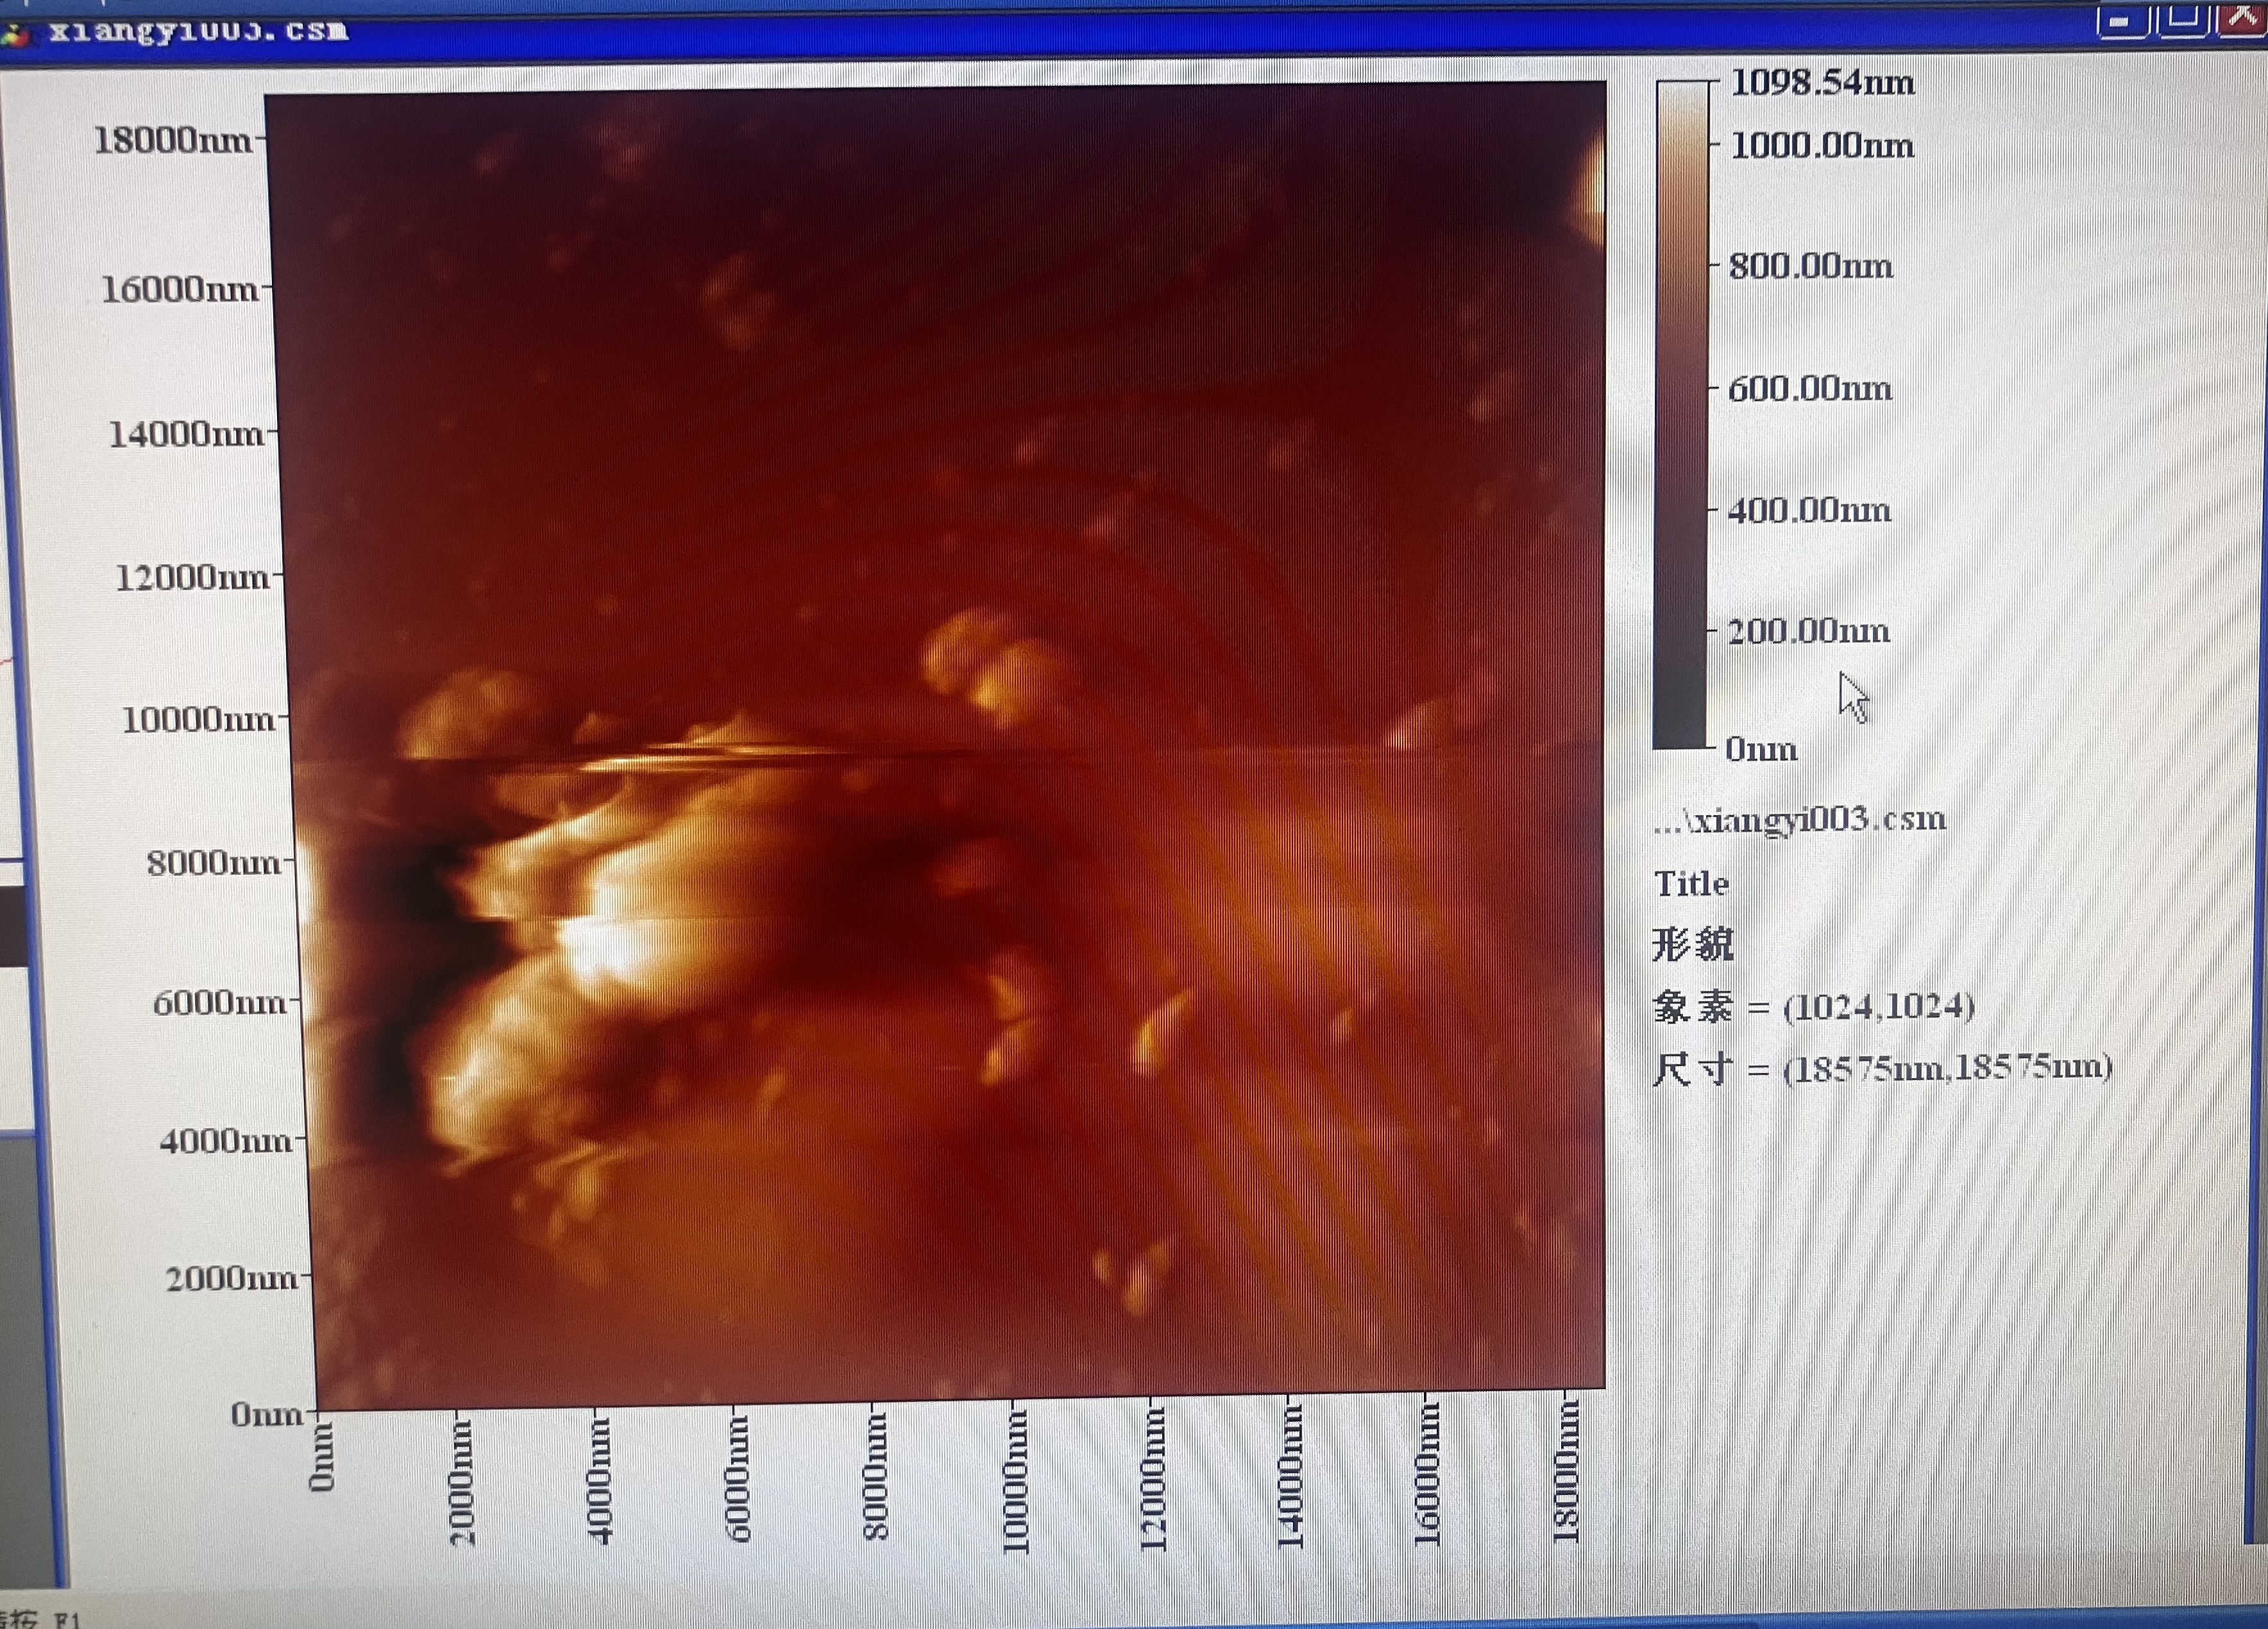
\includegraphics[width=0.9\textwidth]{2.JPG}\\
    {\small{
        图2. 2D形貌灰度图像
    }}
    \vspace{10pt}
\end{minipage}
\begin{minipage}[!ht]{0.5\linewidth}
    \centering
    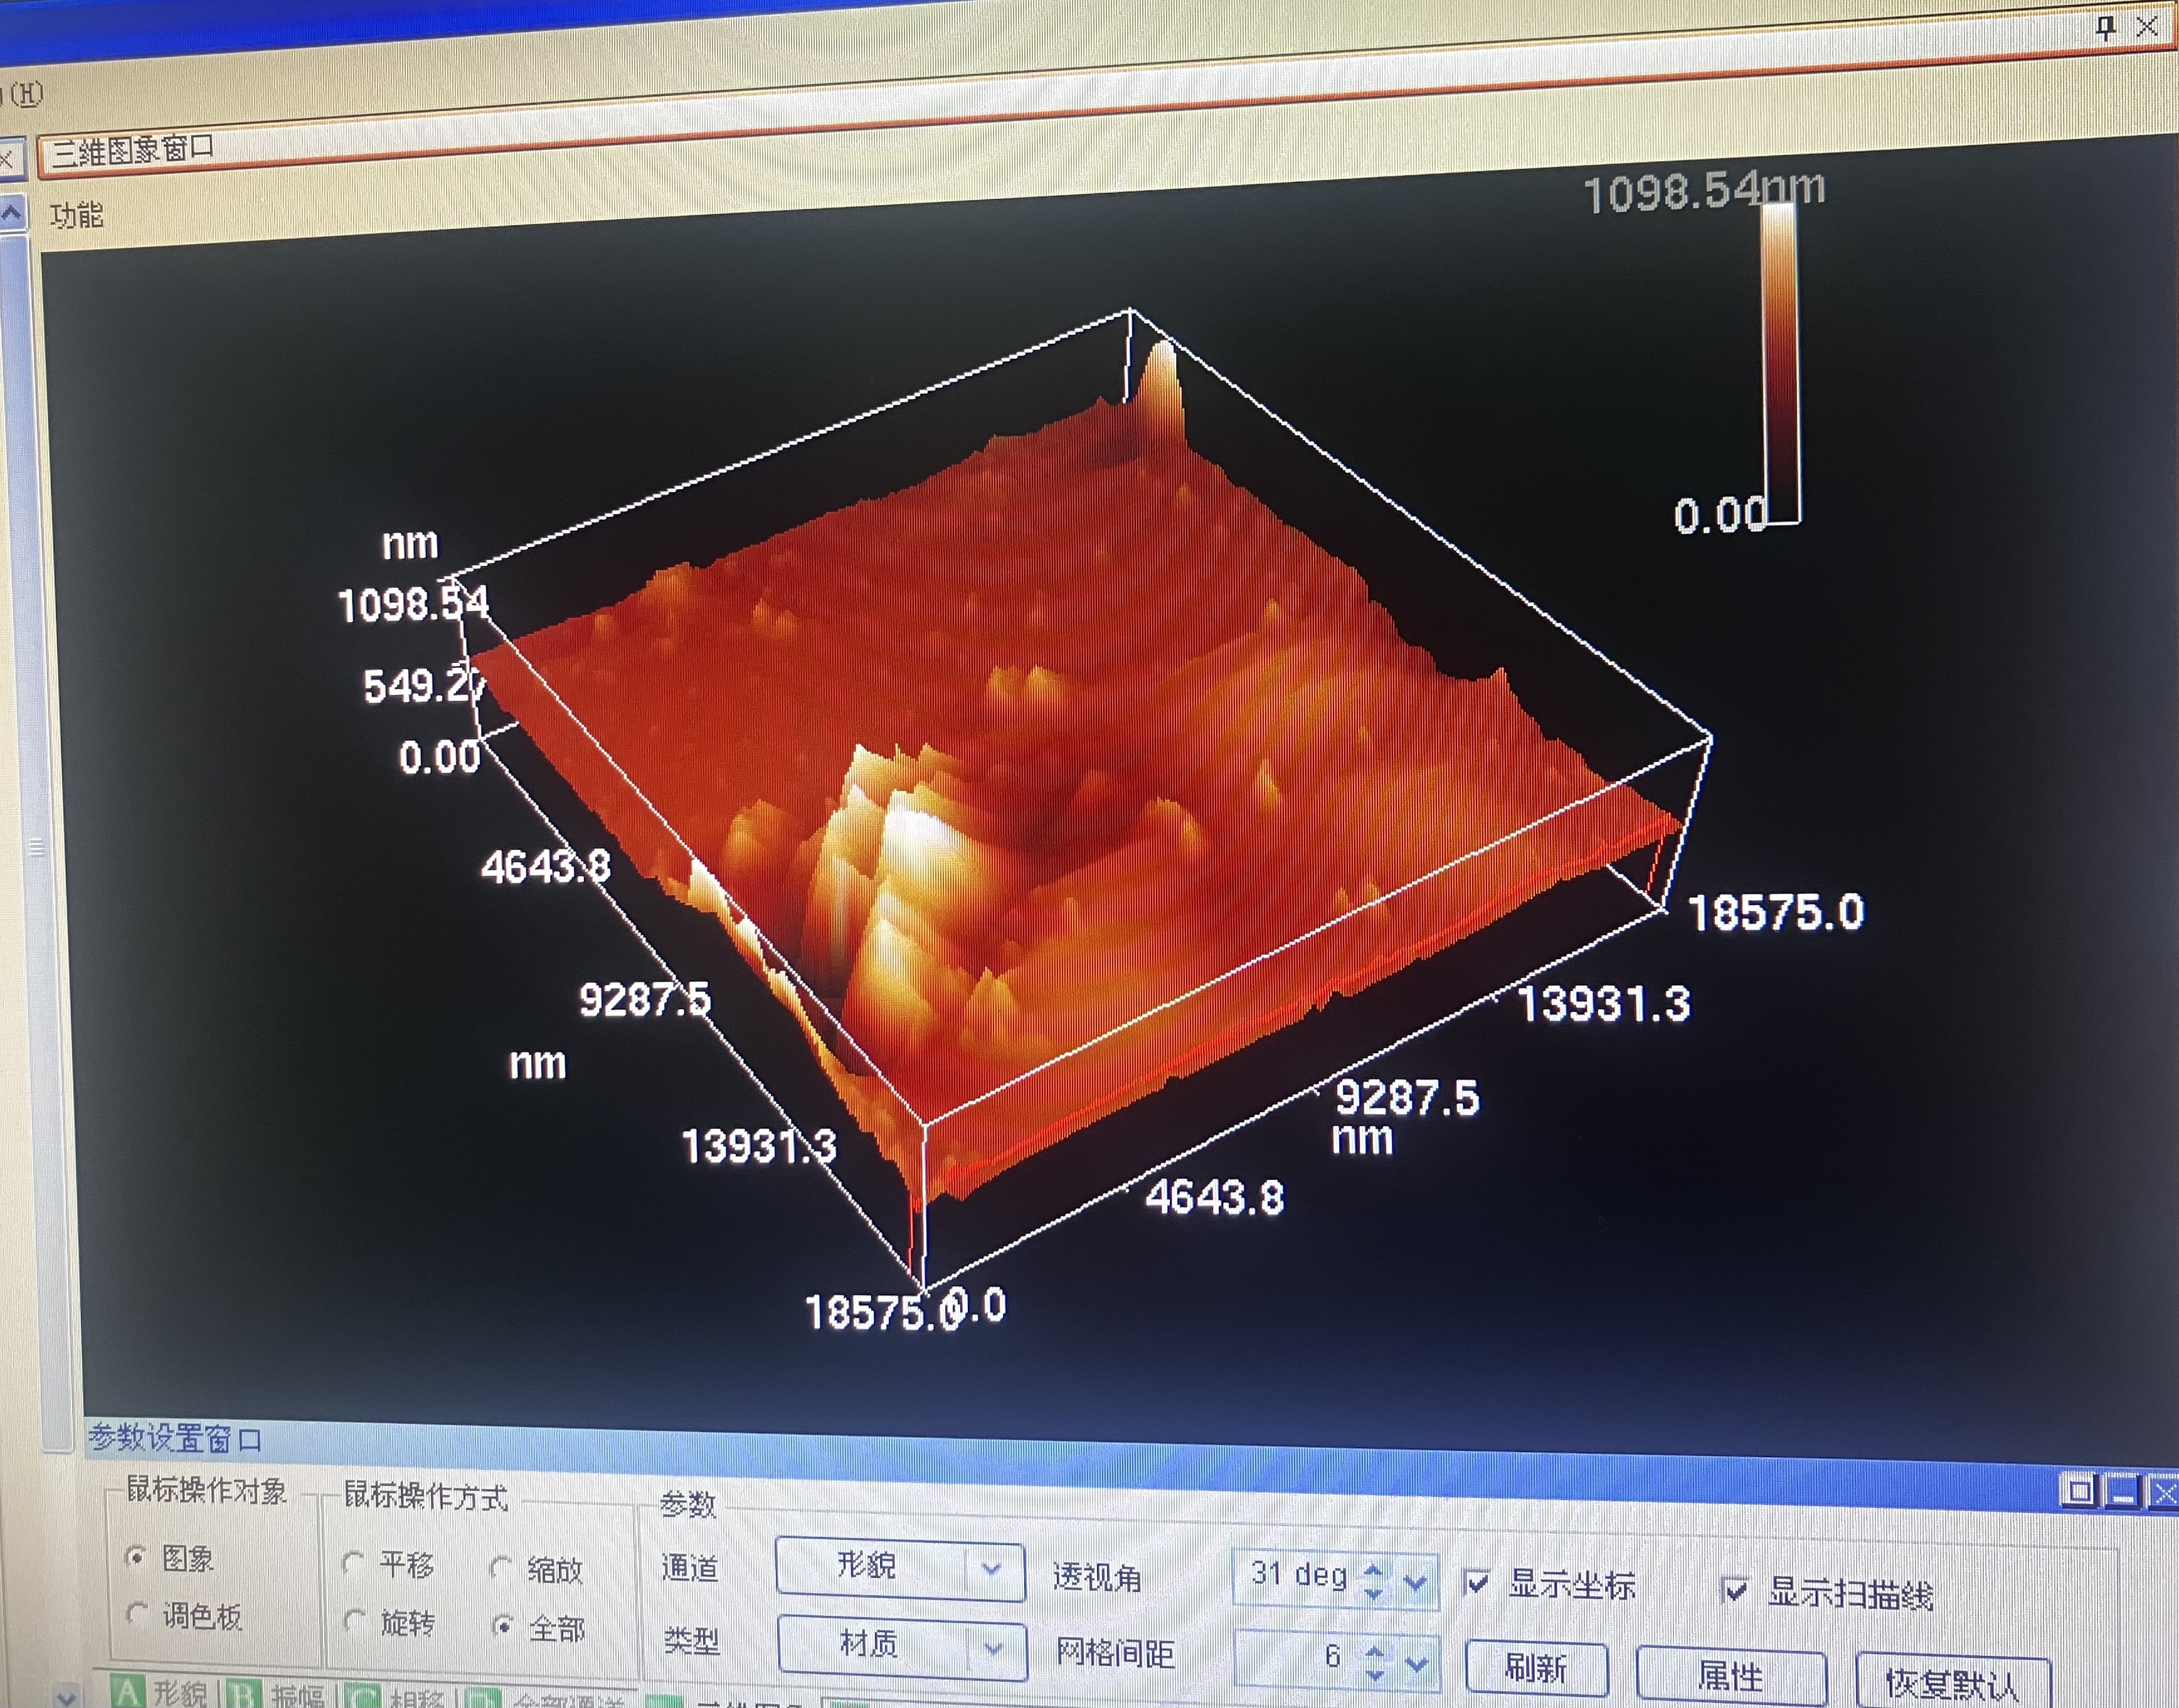
\includegraphics[width=0.9\textwidth]{3.JPG}\\
    {\small{
        图3. 3D形态图像
    }}
    \vspace{10pt}
\end{minipage}\\
\begin{minipage}[!ht]{0.5\linewidth}
    \centering
    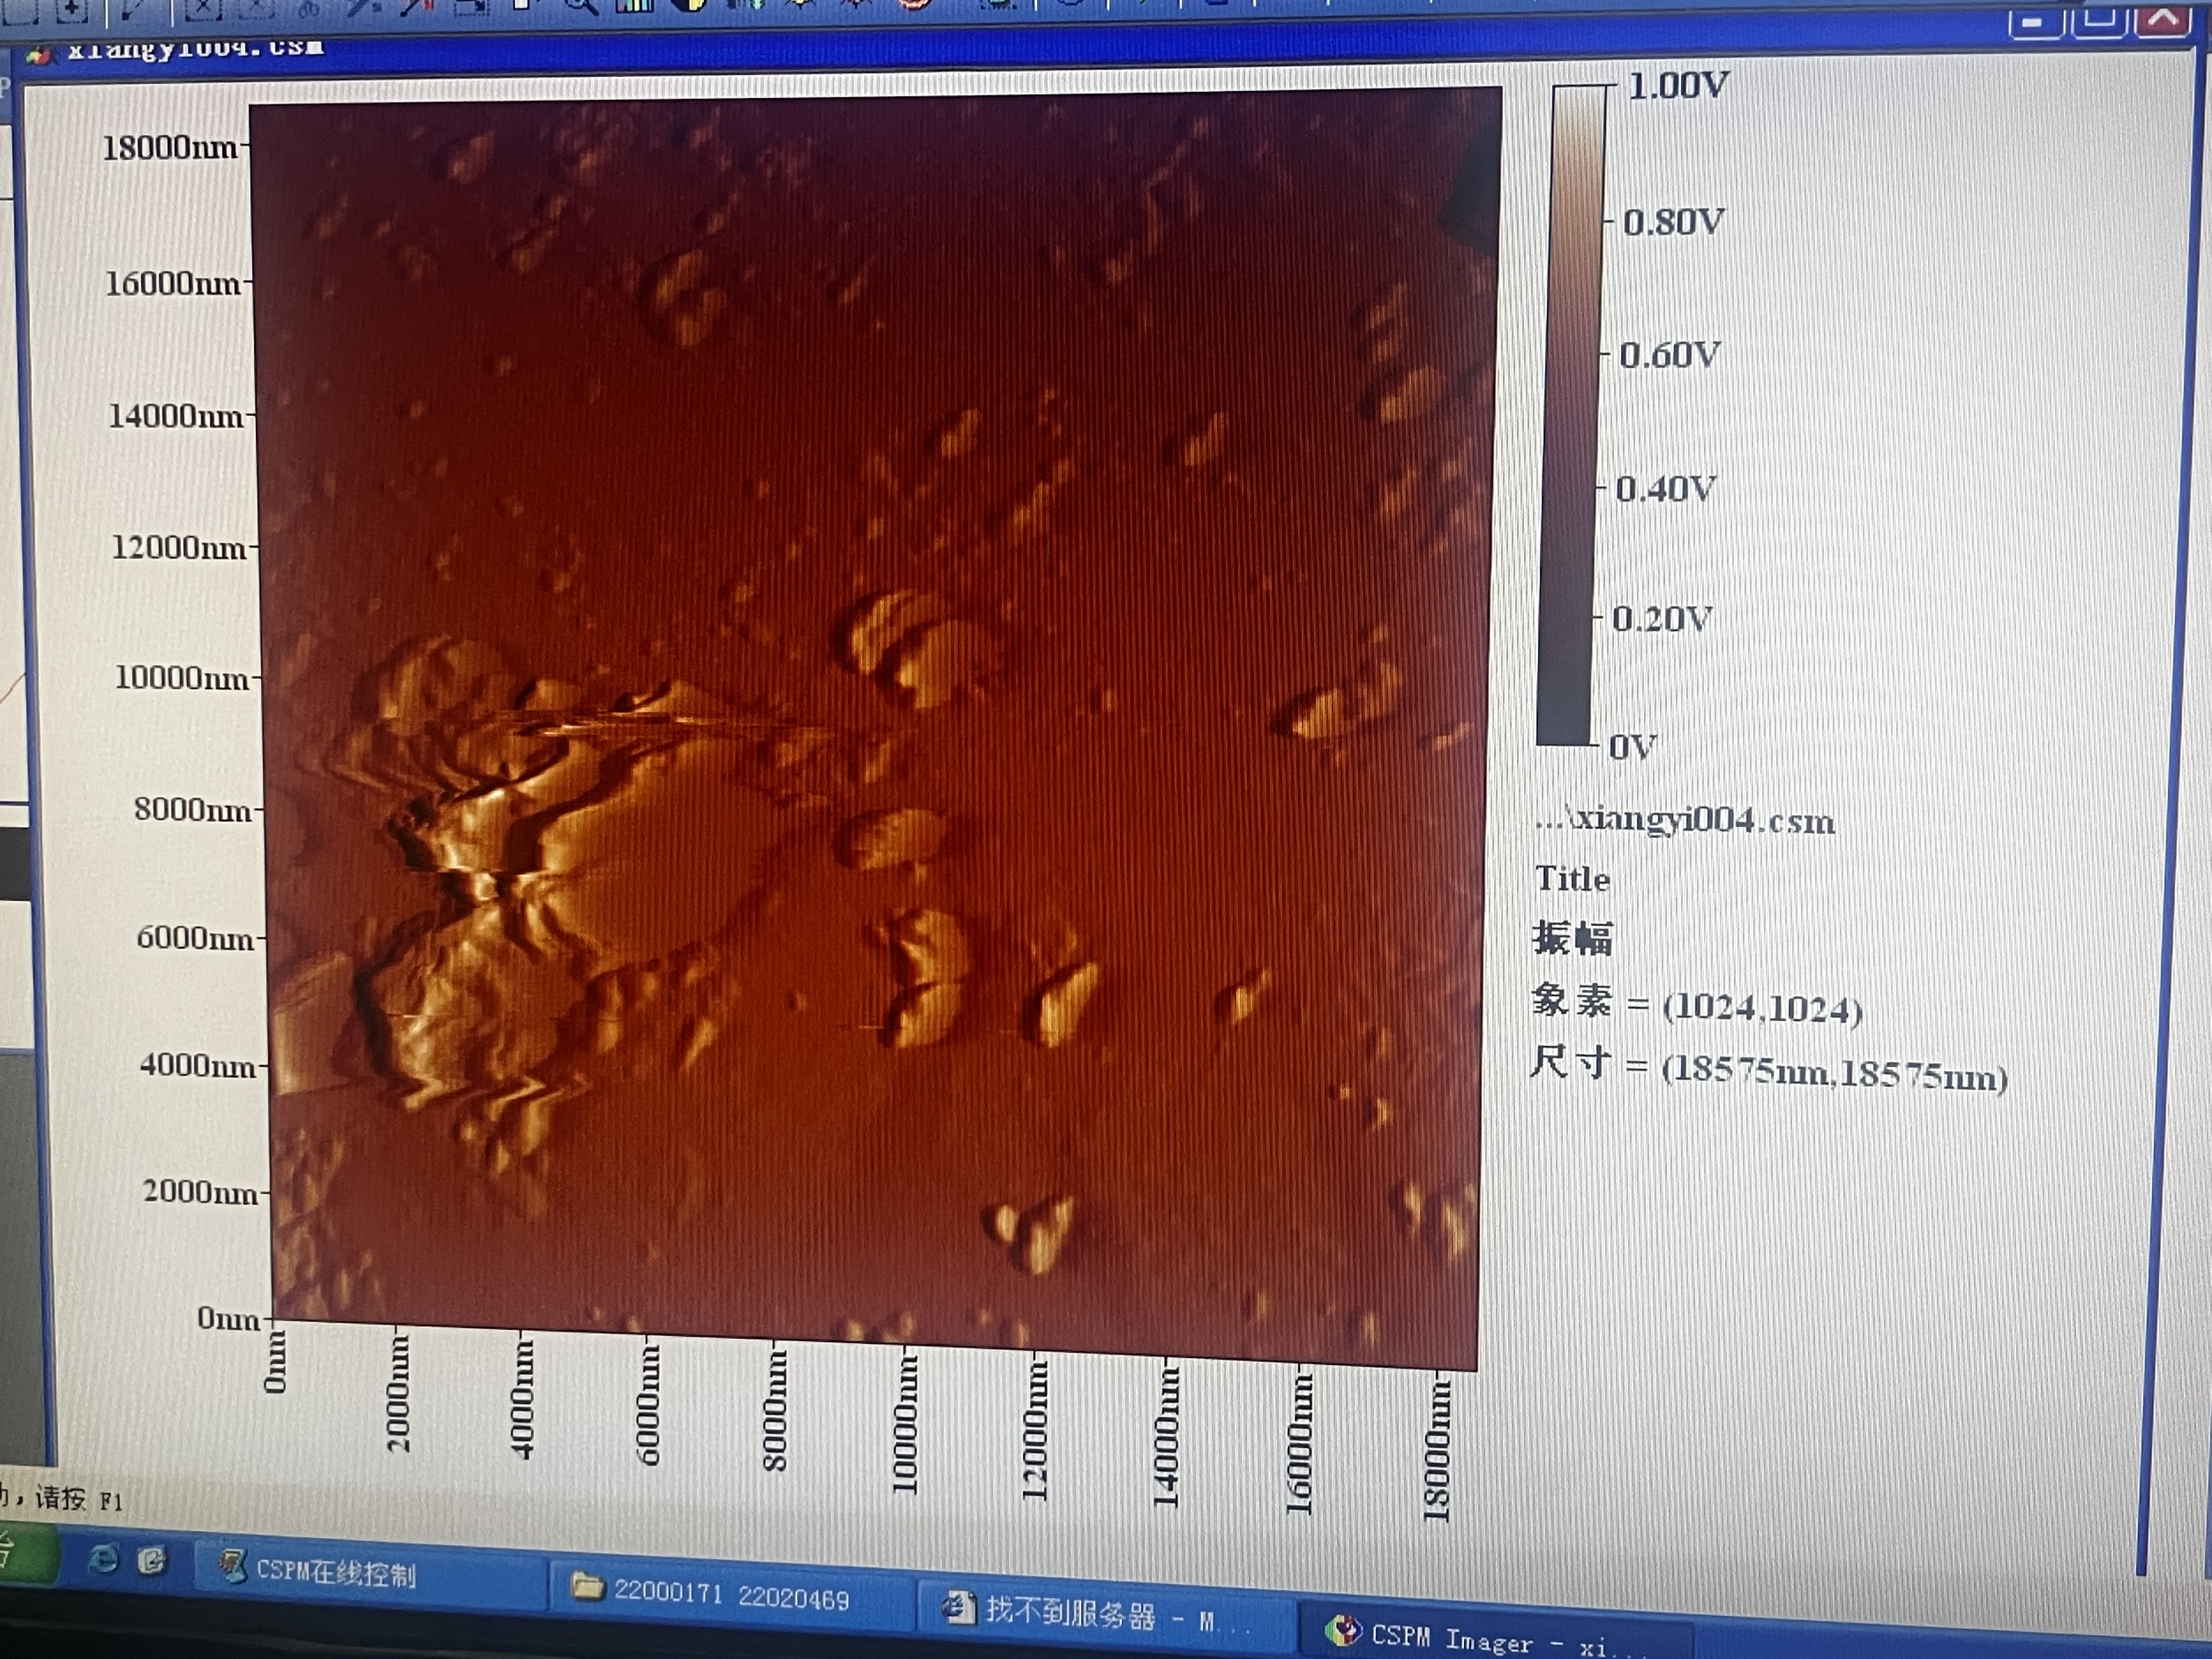
\includegraphics[width=0.9\textwidth]{4.JPG}\\
    {\small{
        图4. 2D振幅灰度图像
    }}
    \vspace{10pt}
\end{minipage}
\begin{minipage}[!ht]{0.5\linewidth}
    \centering
    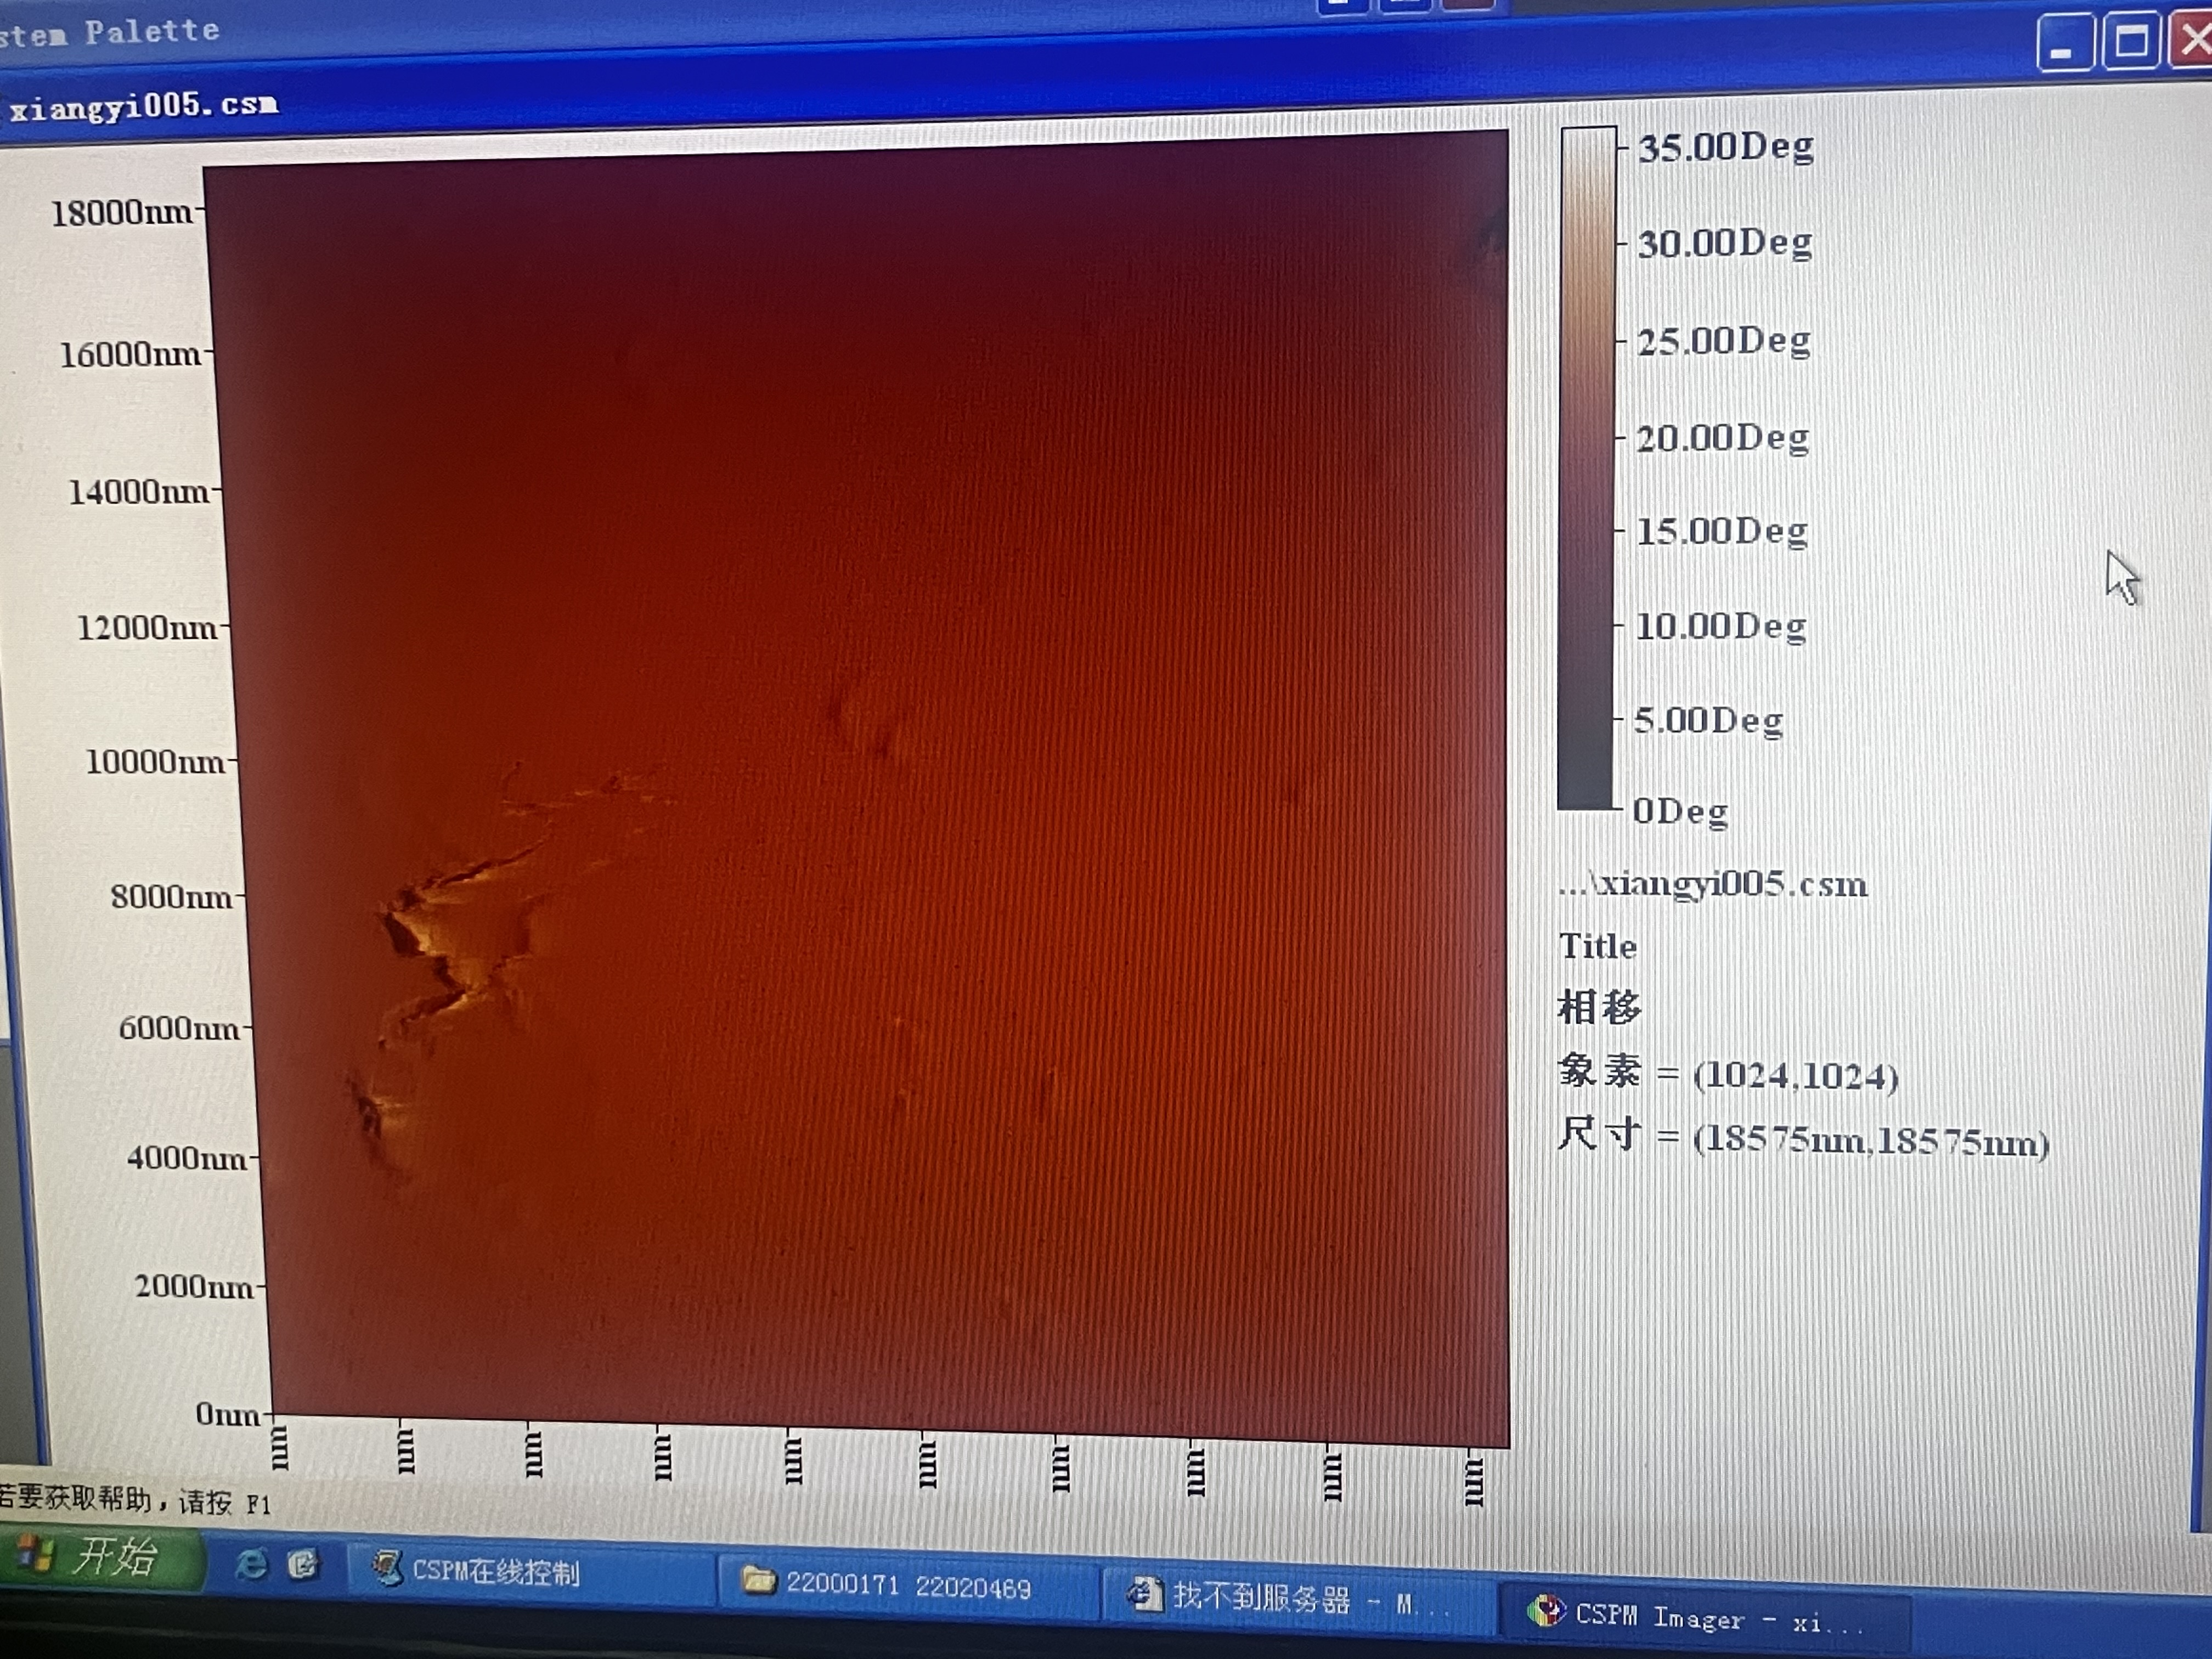
\includegraphics[width=0.9\textwidth]{5.JPG}\\
    {\small{
        图5. 2D相移灰度图像
    }}
    \vspace{10pt}
\end{minipage}\\
\section{结论}
\begin{enumerate}
    \item 本实验利用激光反馈以及反馈电路控制样品表面的扫描,具有较高的精度.
    \item 扫描的时候出现了类似涂抹的现象, 这是出于探针受到外部干扰出现晃动产生的误差, 而不是永久损伤. 首先因为只有x方向出现误差, 如果是探针损伤则应当在y方向也出现误差. 其次是由于扫描方式选择的是轻敲模式, 损伤的概率很小. 之后若扫描图像出现类似现象时, 应当提高工作台的稳定性, 以减少误差.
\end{enumerate}
\subsection{思考题}
\begin{enumerate}
    \item 扫描隧道显微镜的工作原理是什么?什么是量子隧道效应?\par 量子隧道效应: 在有限高势垒中, 粒子即使能量比势能低也依然有可能通过势垒. STM中, 针尖接近样品表面并施加电压, 于是电子由于量子隧道效应从针尖隧穿到样品. STM可以测量这个隧道电流并以此得到针尖与样品的距离.\\
    \item 扫描隧道显微镜主要常用的有哪几种扫描模式?各有什么特点?\par 恒流模式: STM保持隧道电流恒定, 调节针尖与样品的具体. 特点: 分辨率高, 适合观察表面相貌.\par 恒高模式: 保持针尖与样品的距离, 记录电流生成图像. 特点: 扫描速度快, 可能导致针尖损坏.\\
    \item 仪器中加在针尖与样品间的偏压是起什么作用的?针尖偏压的大小对实验结果有何影响?\par 偏压影响隧道电流的大小和方向. 偏压过高会导致电流过大, 针尖更可能损坏. 偏压过低导致信噪比低, 分辨率差.
    \item 实验中隧道电流设定的大小意味着什么?\par 意味着针尖与样品的电子密度, 隧道电流越大表示针尖离样品更近. 
    \item 原子力显微镜的工作原理是什么?\par 通过探针和样品表面的范德华力, 使悬臂出现弯曲. 用激光照射悬臂并检测反射光, 就可以精确测量探针悬臂的弯曲程度, 进而探测探针和样品表面的具体. 接触模式下探针始终与样品接触, 非接触模式下探针在上方振动, 轻敲模式下探针在表面附近振动, 既避免了接触模式对探针和样品的损伤, 精度也高于非接触模式.
\end{enumerate}
\section{致谢}
感谢王中平老师和助教老师细致明确教学讲解和对操作中问题的不倦地答疑! 感谢大学物理实验教学中心提供的仪器!
\section{参考文献}
[1] 大学物理实验教学中心. 扫描探针显微镜实验讲义. 2024;\par
[2] Hiroyuki Mogi, Rin Wakabayashi, Shoji Yoshida, Yusuke Arashida, Atsushi Taninaka, Katsuya Iwaya, Takeshi Miura, Osamu Takeuchi, Hidemi Shigekawa. Time-resolved force microscopy using the delay-time modulation method. Applied Physics Express, 2024;\par
[3] Lalith Krishna Samanth Bonagiri, Zirui Wang, Shan Zhou, Yingjie Zhang. Precise Surface Profiling at the Nanoscale Enabled by Deep Learning. Nano Letters, 2024;\par
\end{document}
